\documentclass[../main.tex]{subfiles}

\begin{document}

\problem{1}

\problempart{a} 
Derive the Hugoniot Eqution.

\assumptions{}
1-D, steady flow.
Inviscid.
Calorically perfect gas (constant specific heats).
Uniform pressure distribution around the CV.
No heat addition (adiabatic).
No work done on or by the CV.

\solution{}

Beginning with the 1-D continuity equation and expressing both velocities in terms of the densities and the other velocity:

\[
    \rho_1 u_1 = \rho_2 u_2
\]

\[
    u_1 = u_2 \left({\frac{\rho_2}{\rho_1}}\right)
\]

\[
    u_2 = u_1 \left({\frac{\rho_1}{\rho_2}}\right)
\]

The 1-D momentum equation:

\[
    p_1 + \rho_1 u_1^2 = p_2 + \rho_2 u_2^2    
\]

Plugging in velocities in terms of 1-D continuity and rearranging:

\[
    p_1 + \rho_1 u_1^2 = p_2 + \rho_2 \left[{u_1 \left({\frac{\rho_1}{\rho_2}}\right)}\right]^2
\]

\[
    (p_1-p_2) =  u_1^2 \left[{\rho_2 \left({\frac{\rho_1}{\rho_2}}\right)^2 - \rho_1}\right]
\]

\[
    (p_1-p_2) = u_1^2 \left[{\left({\frac{\rho_1^2}{\rho_2}}\right) - \rho_1}\right]
\]

\[
    (p_1-p_2) = u_1^2 \left({\frac{\rho_1}{\rho_2}}\right) \left({\rho_1-\rho_2}\right)
\]

We now have relationships for \(u_1\) and \(u_2\) in terms of pressures and densities.

\[
    u_1^2 = \left({\frac{p_1-p_2}{\rho_1-\rho_2}}\right) \left({\frac{\rho_2}{\rho_1}}\right)
\]

\[
    u_2^2 = \left({\frac{p_2-p_1}{\rho_2-\rho_1}}\right) \left({\frac{\rho_1}{\rho_2}}\right)
\]

Next, the 1-D energy equation (adiabatic, no work):

\[
    h_1 + \frac{u_1^2}{2} = h_2 + \frac{u_2^2}{2} 
\]    

The definition of enthalpy, \(h\).

\[
    h = e + \frac{p}{\rho}    
\]

Recasting the 1-D energy equation with the definition of enthalpy and rearranging:

\[
    e_1 + \frac{p_1}{\rho_1} + \frac{u_1^2}{2} = e_2 + \frac{p_2}{\rho_2} + \frac{u_2^2}{2} 
\] 

\[
    e_1 + \frac{p_1}{\rho_1} + \frac{1}{2} \left[{\left({\frac{p_1-p_2}{\rho_1-\rho_2}}\right) \left({\frac{\rho_2}{\rho_1}}\right)}\right] =\
    e_2 + \frac{p_2}{\rho_2} + \frac{1}{2} \left[{\left({\frac{p_2-p_1}{\rho_2-\rho_1}}\right) \left({\frac{\rho_1}{\rho_2}}\right)}\right]
\] 


\[
   0  =  \left({e_2 - e_1}\right) + \left({\frac{p_2}{\rho_2}-\frac{p_1}{\rho_1}}\right) + 
   \frac{1}{2} \left[{\left({\frac{p_2-p_1}{\rho_2-\rho_1}}\right) \left({\frac{\rho_1}{\rho_2} - \frac{\rho_2}{\rho_1}}\right)}\right]
\]

\[
   0  =  \left({e_2 - e_1}\right) + \left({\frac{p_2\rho_1 - p_1\rho_2}{\rho_1\rho_2}}\right) + 
   \frac{1}{2} \left[{\left({\frac{p_2-p_1}{\rho_2-\rho_1}}\right) \left({\frac{\rho_1^2-\rho_2^2}{\rho_1\rho_2}}\right)}\right]
\]

\[
   0  =  \left({e_2 - e_1}\right) + 
   \left({\frac{1}{\rho_1\rho_2}}\right)
   \left[{
    \left({p_2\rho_1 - p_1\rho_2}\right) +
    \frac{1}{2} \left({\frac{p_2-p_1}{\rho_2-\rho_1}}\right) \left({\rho_1^2-\rho_2^2}\right)
   }\right]
\]

\[
    0  =  \left({e_2 - e_1}\right) + 
    \left({\frac{1}{\rho_1\rho_2}}\right)
    \left[{
    \left({p_2\rho_1 - p_1\rho_2}\right) +
    \frac{1}{2} \left({\frac{p_1-p_2}{\rho_1-\rho_2}}\right) \left({\rho_1-\rho_2}\right) \left({\rho_1+\rho_2}\right)
    }\right]
\]

\[
    0  =  \left({e_2 - e_1}\right) + 
    \left({\frac{1}{\rho_1\rho_2}}\right)
    \left[{
    \left({p_2\rho_1 - p_1\rho_2}\right) +
    \frac{1}{2} \left({p_1-p_2}\right) \left({\rho_1+\rho_2}\right)
    }\right]
\]

\[
    0  =  \left({e_2 - e_1}\right) + 
    \left({\frac{1}{\rho_1\rho_2}}\right)
    \left[{
    \left({p_2\rho_1 - p_1\rho_2}\right) +
    \frac{1}{2} \left({p_1\rho_1 + p_1\rho_2 - p_2\rho_1 -p_2\rho_2}\right)
    }\right]
\]

\[
    0  =  \left({e_2 - e_1}\right) + 
    \left({\frac{1}{2}}\right)
    \left({\frac{1}{\rho_1\rho_2}}\right)
    \left({p_1\rho_1 - p_1\rho_2 + p_2\rho_1 -p_2\rho_2}\right)
\]

\[
    \left({e_2 - e_1}\right) =
    \left({\frac{1}{2}}\right)
    \left({\frac{p_1}{\rho_2} - \frac{p_1}{\rho_1} + \frac{p_2}{\rho_2} - \frac{p_2}{\rho_1}}\right)
\]

\[
    \left({e_2 - e_1}\right) =
    \left({\frac{p_1 + p_2}{2}}\right)
    \left({\frac{1}{\rho_1} - \frac{1}{\rho_2}}\right)
\]

We now have one of the common forms of the Hugoniot Equation:

\[
    \left({e_2 - e_1}\right) =
    \left({\frac{p_1 + p_2}{2}}\right)
    \left({\nu_1 - \nu_2}\right)
\]

For a CPG, internal energy, \(e\):

\[
    e = c_\nu T
\]   

Substituting the above relationship into our initial Hugoniot Equation:

\[
    c_\nu \left({T_2 - T_1}\right) =
    \left({\frac{p_1 + p_2}{2}}\right)
    \left({\nu_1 - \nu_2}\right)
\]

For a CPG, \(c_\nu\):

\[
    c_\nu = \frac{R}{\gamma-1}
\] 

Substituting and rearranging:

\[
    \frac{R}{\gamma-1} \left({T_2 - T_1}\right) =
    \left({\frac{p_1 + p_2}{2}}\right)
    \left({\nu_1 - \nu_2}\right)
\]

The ideal gas equation of state:

\[
    T = \frac{p \nu}{R}
\]    

Substituting and rearranging to solve for \(p_2/p_1\):

\[
    \frac{R}{\gamma-1} \left({\frac{p_2 \nu_2}{R} - \frac{p_1 \nu_1}{R}}\right) =
    \left({\frac{p_1 + p_2}{2}}\right)
    \left({\nu_1 - \nu_2}\right)
\]

\[
    \frac{2}{\gamma-1} \left({p_2 \nu_2 - p_1 \nu_1}\right) =
    \left({p_1 + p_2}\right)
    \left({\nu_1 - \nu_2}\right)
\]

\[
    \frac{2}{\gamma-1} \left({p_2 \nu_2 - p_1 \nu_1}\right) =
    p_1 \nu_1 - p_1 \nu_2 + p_2 \nu_1 - p_2 \nu_2
\]

\[
    \left({\frac{2}{\gamma-1} + 1}\right) \left({p_2 \nu_2 - p_1 \nu_1}\right) =
    \left({p_2 \nu_1 - p_1 \nu_2}\right)
\]

\[
    \left({\frac{\gamma+1}{\gamma-1}}\right)  =
    \frac{\left({p_2 \nu_1 - p_1 \nu_2}\right)}
    {\left({p_2 \nu_2 - p_1 \nu_1}\right)}
\]

\[
    \left({\frac{\gamma+1}{\gamma-1}}\right)  =
    \frac{\left({\frac{p_2}{p_1} \nu_1 - \nu_2}\right)}
    {\left({\frac{p_2}{p_1} \nu_2 - \nu_1}\right)}
\]

\[
    \left({\frac{\gamma+1}{\gamma-1}}\right) {\left({\frac{p_2}{p_1} \nu_2 - \nu_1}\right)}  =
    \left({\frac{p_2}{p_1} \nu_1 - \nu_2}\right)
\]

\[
    \left({\frac{\gamma+1}{\gamma-1}}\right) {\left({\frac{p_2}{p_1} \nu_2 - \nu_1}\right)}  =
    \left({\frac{p_2}{p_1} \nu_1 - \nu_2}\right)
\]

\[
    \frac{p_2}{p_1} \left[{\left({\frac{\gamma+1}{\gamma-1}}\right) \nu_2 - \nu_1 }\right] =
    \left({\frac{\gamma+1}{\gamma-1}}\right) \nu_1 - \nu_2
\]

\[
    \frac{p_2}{p_1} = \left[{
        \frac{\left({\frac{\gamma+1}{\gamma-1}}\right) \nu_1 - \nu_2}{{\left({\frac{\gamma+1}{\gamma-1}}\right) \nu_2 - \nu_1 }}
    }\right]
\]

\[
    \frac{p_2}{p_1} = \left[{
        \frac{\left({\frac{\gamma+1}{\gamma-1}}\right) \frac{\nu_1}{\nu_2} - 1}{{\left({\frac{\gamma+1}{\gamma-1}}\right) - \frac{\nu_1}{\nu_2} }}
    }\right]
\]

The relation between density, \(\rho\), and specific volume, \(\nu\):

\[
    \rho = \frac{1}{\nu}
\]

Substituting the above relation yields the final form of the Hugoniot Equation for pressure ratio across a normal shock in terms of density ratio and \(\gamma\):

\[
    \boxed{
    \frac{p_2}{p_1} = \left[{
        \frac{\left({\frac{\gamma+1}{\gamma-1}}\right) \frac{\rho_2}{\rho_1} - 1}{{\left({\frac{\gamma+1}{\gamma-1}}\right) - \frac{\rho_2}{\rho_1} }}
    }\right]
    }
\]

\problempart{b}

Assume that a turbojet compressor fan isentropically compresses air for a range 1 \(<\) \(\frac{\rho_2}{\rho_1}\) \(<\) 5. 
Plot the compression (i.e., \(\frac{p_2}{p_1}\)) for this range of \(\frac{\rho_2}{\rho_1}\) for both traditional isentropic compression (e.g., a turbojet compression fan) and normal-shock-wave compression. 
These curves should be on the same plot with a clearly labeled legend.

\givens{}
Isentropic and normal shock compression of air.
\(1 < \frac{\rho_2}{\rho_1} < 5\).

\assumptions{}
Inviscid, adiabatic, no external work. Air is a CPG with \(\gamma =1.4\).

\solution{}
\textit{Note: All calculations performed in Python, see Appendix \ref{Problem1Python}}.
The static pressure ratio across a normal shock given by the Hugoniot equation:

\[
    \frac{p_2}{p_1} = \left[{
        \frac{\left({\frac{\gamma+1}{\gamma-1}}\right) \frac{\rho_2}{\rho_1} - 1}{{\left({\frac{\gamma+1}{\gamma-1}}\right) - \frac{\rho_2}{\rho_1} }}
    }\right]
\]

The static pressure ratio given as a function of density ratio for isentropic compression:

\[
    \frac{p_2}{p_1} = \left({\frac{\rho_2}{\rho_1}}\right)^\gamma
\]

Figure \ref{compression} shows a comparison of the compression (pressure ratio) as a function of density ratio for both isentropic compression and normal shock compression.

\begin{figure}[h!]
    \centering
    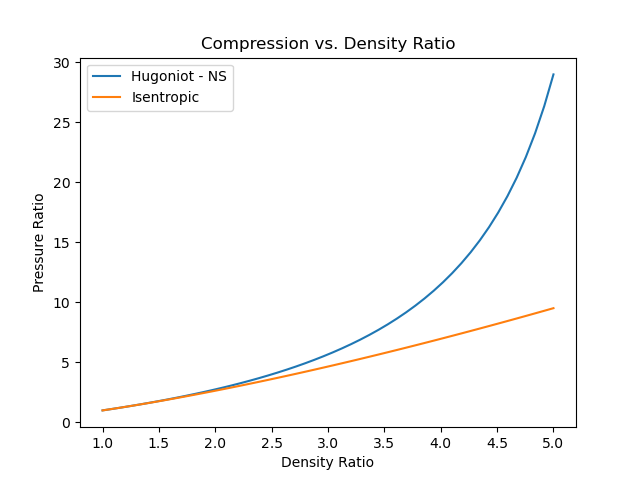
\includegraphics[scale=0.75]{../../images/problem_1/hugoniot_vs_isentropic_compression.png}
    \caption{Compression vs. density ratio -- normal shock and isentropic compression}
    \label{compression}
\end{figure}

\newpage

\problempart{c} 

If you were tasked with deciding which mechanism to use to compress air, which would you choose? 
For relatively large \(\frac{\rho_2}{\rho_1}\), what other real-world considerations are there for choosing between isentropic versus normal-shock-wave compression? 
Think of “efficiency”.

\discussion{}

The normal shock wave delivers much higher static pressure ratios for relatively large density ratios. 
Absent other context, the normal shock appears to be the ideal solution.
However, normal shocks generate large total pressure losses, which are a measure of efficiency.
Isentropic compression does not deliver pressure ratios as large as normal shocks, but they are not lossy by definition.
Figure \ref{efficiency} shows the total pressure ratio across a normal shock as a function of incoming Mach number.
Total pressure ratio plummets as incoming Mach number increases. 
By approximately Mach 2.5, the flow has lost half of its total pressure because of the presence of a normal shock.
For hypersonic Mach numbers (5+), the total pressure recovery is around 10\% or less!
When the density ratio associated with a compression process is approximately 2.5 or less, both methods of compression deliver approximately the same pressure ratio.
Isentropic compression methods require turbomachinery and moving parts which contribute substantial amounts of weight to a vehicle.
If the losses are acceptable, normal shock compression at an inlet could be a potentially desirable design choice for minimizing weight.

\begin{figure}[h!]
    \centering
    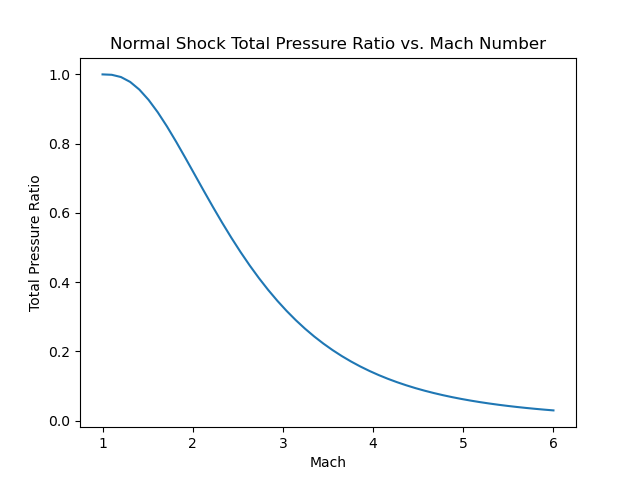
\includegraphics{../../images/problem_1/compression_efficiency_NS.png}
    \caption{Compression vs. Mach number across normal shock}
    \label{efficiency}
\end{figure}

\newpage

\problempart{d}

Calculate the change in entropy \((s_2 - s_1)\) from the given range of \(\frac{\rho_2}{\rho_1}\) for both the isentropic and normal-shock compression. 
Plot \((s_2 - s_1)\) versus \(\frac{\rho_2}{\rho_1}\) , and comment on what you find.
Does this affect your thoughts on part (c)? 
Research, and then briefly explain, the physical explanation for the \((s_2 - s_1)\) behavior across the normal shock.

\givens{}
Isentropic and normal-shock compression.

\assumptions{}
Air is a CPG with \(\gamma=1.4\).

\solution{}

By definition, \((s_2 - s_1)\) for isentropic flow should be equal to 0.
For a CPG, Gibb's equation:

\[
    s_2 - s_1 = c_p \ln{\left({\frac{T_2}{T_1}}\right)} - R \ln{\left({\frac{p_2}{p_1}}\right)}
\]

Recasting the temperature ratio in terms of the density ratio using isentropic relations:

\[
    \frac{T_2}{T_1} = \left({\frac{\rho_2}{\rho_1}}\right)^{\gamma-1}
\]

\[
    s_2 - s_1 = c_p \ln{\left({\left({\frac{\rho_2}{\rho_1}}\right)^{\gamma-1}}\right)} - R \ln{\left({\frac{p_2}{p_1}}\right)}
\]

The change in density across a normal shock:

\[
    s_2 - s_1 = -R \ln {\frac{p_{t,2}}{p_{t,1}}}
\]

Solving for \(\frac{p_{t,2}}{p_{t,1}}\) across a normal shock is a multi-step process.
Beginning with the pressure ratios calculated in part (b) using the Hugoniot Equation, we can solve for upstream Mach number.

\[
    \frac{p_2}{p_1} = 1 + \frac{2\gamma}{\gamma+1}\left(M_1^2-1\right)
\]

\[
    M_1 = \sqrt{\left({\frac{p_2}{p_1} - 1}\right)\left({\frac{\gamma+1}{2\gamma}}\right) + 1}
\]

Next, the total pressure ratio across a normal shock is given by the following equation:

\[
    \frac{p_{t,2}}{p_{t,1}} = 
    \frac{p_{t,2}}{p_2} \frac{p_2}{p_1} \frac{p_1}{p_{t,1}} =
    {\left[{
    \frac{\frac{\gamma+1}{2}M_1^2}
    {1 + \frac{\gamma-1}{2}M_1^2}
    }\right]}^ {\frac{\gamma}{\gamma-1}}
    \left[{
    \frac{2\gamma}{\gamma+1}M_1^2 - \frac{\gamma-1}{\gamma+1}
    }\right]^{\frac{1}{1-\gamma}}
\]

Figure \ref{entropy} shows the entropy change for both compression methods.
As initially presumed, the isentropic compression by definition has no entropy change.
The normal shock compression has non-zero entropy change, increasing with density ratio.
Shocks are highly lossy in a very thin region, although flow up and downstream can generally be considered isentropic.
The near-instantaneous change in flow properties across the thin shock-region cannot be considered ``reversible'', therefore any work-related assumptions are rendered invalid.
The entropy change increases with density ratio because the shock strength required to generate that density ratio is also increasing, and stronger shocks (associated with higher Mach flows) are lossier and less efficient.
The results shown here support the discussion in part (c), indicating that losses are a major factor in normal shock compression.

\begin{figure}[h!]
    \centering
    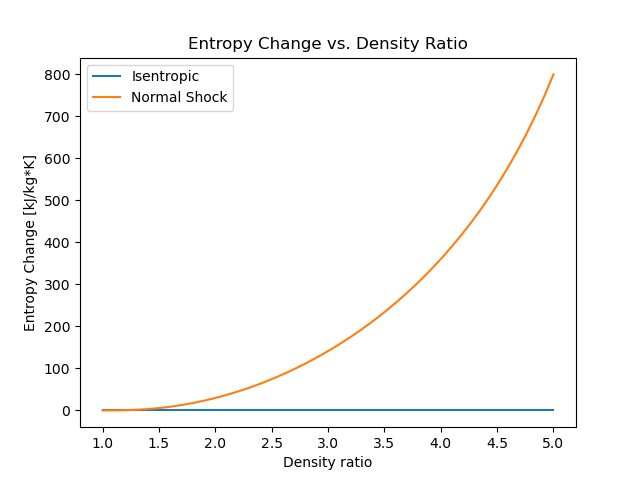
\includegraphics{../../images/problem_1/entropy_change.png}
    \caption{Entropy change for normal-shock and isentropic compression}
    \label{entropy}
\end{figure}

\newpage

\problempart{e}

Using your figure from part (b), for what range of \(\frac{\rho_2}{\rho_1}\) are the two processes comparable?
Explain why this makes sense. 
For what Mach-number (i.e., M1) range would this correspond to regarding the normal-shock-wave case? 
Does this help you explain?

\discussion{}

Referencing \ref{compression}, the two compression processes are comparable up to approximately \(\frac{\rho_2}{\rho_1} = 2.5\).
From a static pressure ratio standpoint, the processes are nearly identical in output.
Examining the entropy change for this density ratio, the normal shock generates entropic losses but the curve of entropy change has not exploded as it does for larger values of \(\frac{\rho_2}{\rho_1}\).
The range of incoming Mach number, \(M_1\), that this corresponds to is \(1 < M_1 < 1.89\).
Although the flow is supersonic and experiences a normal shock, it is not extremely supersonic and the associated entropy change and total pressure loss for this relatively low value of \(M_1\) are sufficiently small that the two compression methods are comparable.
 

\end{document}